\section{Setting the map projection} \label{subsec:adv_mapproj}
%------------------------------------------------------

In \scalerm, grids are allocated based on actual distance. The latitude and longitude for all grids are calculated by using the latitude and longitude of a certain reference point using a map projection. All information pertaining to the latitude and longitude of the grids are output to all output files in \netcdf format. The locations of the domain and the map projection can be configured in \nmitem{PARAM_MAPPROJECTION}. \textcolor{blue}{This configuration must be shared among the configuration files \texttt{pp.conf}, \texttt{init.conf}, and \texttt{run.conf}.} An example is as follows:
\editboxtwo{
\verb|&PARAM_MAPPROJECTION| & \\
\verb| MAPPROJECTION_basepoint_lon = 138.727778D0,| & \\
\verb| MAPPROJECTION_basepoint_lat = 35.360556D0,|  & \\
\verb| MAPPROJECTION_type          = 'MER',|        & ; Choose from Table \ref{tab:map_proj}.\\
\verb|/| & \\
}

\begin{table}[htb]
\begin{center}
\caption{Map projections selectable in \scalerm}
\begin{tabularx}{150mm}{|l|X|} \hline
 \rowcolor[gray]{0.9} \verb|MAPPROJECTION_type| & Map projection\\ \hline
 \verb|NONE| & No map projection for ideal experiment ( default ) \\ \hline
 \verb|LC|   & Lambert conformal conic projection   \\ \hline
 \verb|PS|   & Polar stereo projection           \\ \hline
 \verb|MER|  & Mercator projection               \\ \hline
 \verb|EC|   & Equi-rectangular projection        \\ \hline
\end{tabularx}
\label{tab:map_proj}
\end{center}
\end{table}

\nmitem{MAPPROJECTION_basepoint_lat, MAPPROJECTION_basepoint_lon} are the latitude and longitude at a reference point. This reference point is the center of the calculation domain by the default setting.
In \scalerm, the north and south latitudes are expressed by positive and negative values, respectively. The east and west longitudes are also expressed by positive and negative values, respectively. It is possible to express longitude using an angle greater than $180^{\circ}$.
In above setting, the center of the domain is configured at $35.360556^{\circ}$N and $138.727778^{\circ}$E, where N and E denote the north latitude and east longitude, respectively. The entire calculation domain is placed at the center with a specified size.

\nmitem{MAPPROJECTION_type} provides the kind of map projection and \verb|MER| the Mercator projection.
Table \ref{tab:map_proj} shows the selectable map projections in the current version of \scalerm. In the case of the Mercator projection, the standard latitude, to which a cylinder is tangent, is specified as \nmitem{MAPPROJECTION_M_lat} in units of degrees. In general, the standard latitude is set to the Equator.
In \scalerm, \nmitem{MAPPROJECTION_basepoint_lat} is used as standard latitude, unless \nmitem{MAPPROJECTION_M_lat} is explicitly specified. This is because this method is more precise with less distortion than the usual Mercator projection.

The text below explains the Lambert conformal conic projection, the usage frequency of which is highest. The example is the same as that in the file used in the tutorial for the real atmospheric experiment.
\editbox{
\verb|&PARAM_MAPPROJECTION| \\
\verb| MAPPROJECTION_basepoint_lon = 135.220404,| \\
\verb| MAPPROJECTION_basepoint_lat = 34.653396,| \\
\verb| MAPPROJECTION_type          = 'LC',| \\
\verb| MAPPROJECTION_LC_lat1       =  30.0,| \\
\verb| MAPPROJECTION_LC_lat2       =  40.0,| \\
\verb|/| \\
}
In \scalerm, two standard parallels are used for this projection.
The north and south of them are specified in \nmitem{MAPPROJECTION_LC_lat1, MAPPROJECTION_LC_lat2} 
in units of degrees.
In the region between the latitudes, the ratio of the latitudinal to longitudinal length is adjusted to be close to the Earth’s ellipsoid face.


Furthermore, it is possible for the reference point (\nmitem{MAPPROJECTION_basepoint_lon},\\
\nmitem{MAPPROJECTION_basepoint_lat}) to be displaced from the default setting, i.e., domain center as follows:

\editbox{
\verb|&PARAM_MAPPROJECTION| \\
\verb| MAPPROJECTION_basepoint_lon = 135.220404,| \\
\verb| MAPPROJECTION_basepoint_lat = 34.653396,| \\
\verb| MAPPROJECTION_basepoint_x   = 100.0,| \\
\verb| MAPPROJECTION_basepoint_y   = 100.0,| \\
\verb| MAPPROJECTION_type          = 'LC',| \\
\verb| MAPPROJECTION_LC_lat1       = 30.0,| \\
\verb| MAPPROJECTION_LC_lat2       = 40.0,| \\
\verb|/| \\
}

The location of the reference point is specified as the distance from the south-west corner (bottom-left corner).;
\nmitem{MAPPROJECTION_basepoint_x} and \nmitem{MAPPROJECTION_basepoint_y} are the distances in units of meters between the south-west corner and the reference point in \XDIR and in \YDIR, respectively.
If they are not specified, the center of projection corresponds to that of the domain.
Figure \ref{fig:map_lc} shows both cases.

\begin{figure}[t]
\begin{center}
  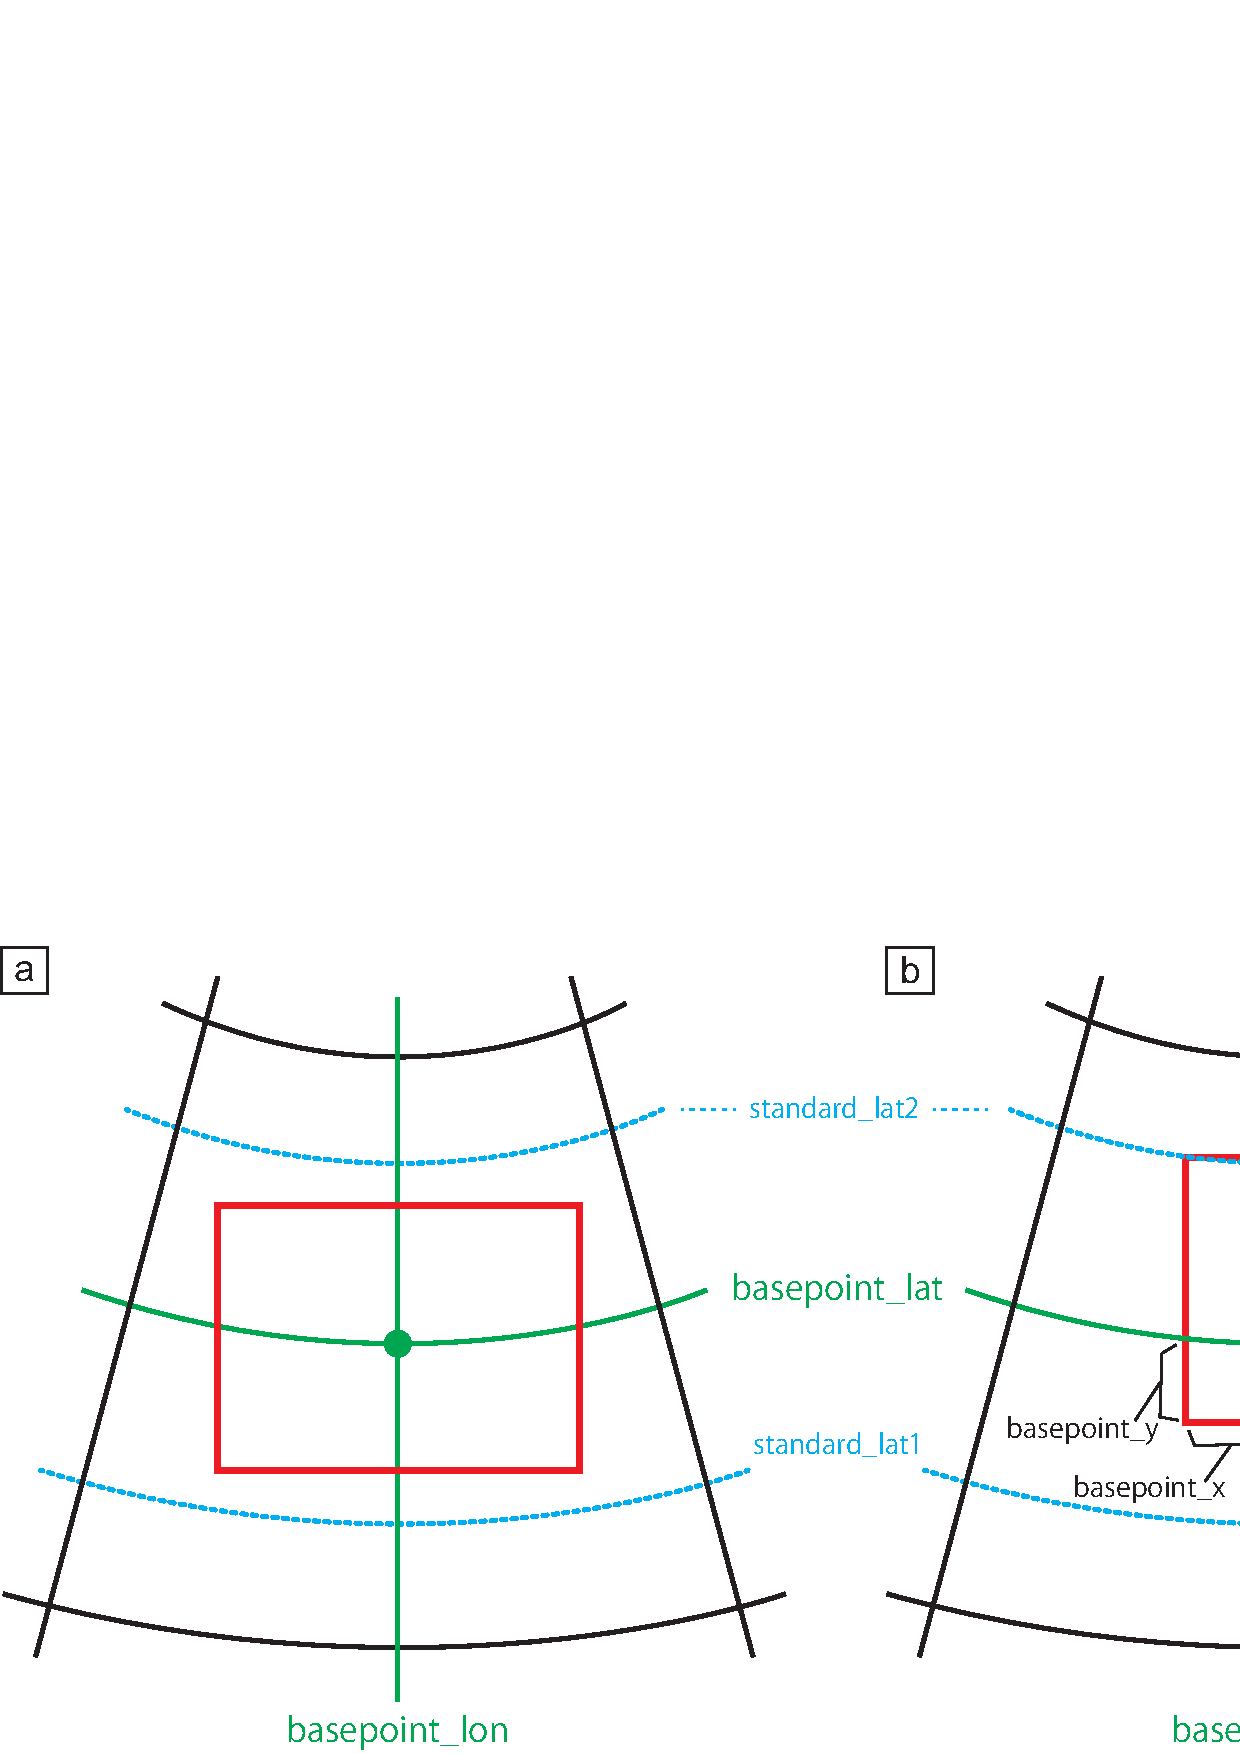
\includegraphics[width=0.8\hsize]{./../../figure/LC_latlon_xy.pdf}\\
  \caption{The relationship between projection center and calculation domain.; (a) Default setting and (b) the case where the center of projection is displaced at the center of the domain.
    The red line indicates the boundary of the calculation domain.}
  \label{fig:map_lc}
\end{center}
\end{figure}

